%%%%
\section{Poluição do ar em cidades}

A poluição do ar ambiental nas cidades dos países em desenvolvimento
guarda algumas similaridades com as cidades dos países desenvolvidos,
ambas possuem fontes poluidoras que são características de meios urbanos, 
se destacando: tráfego de veículos automotivos, indústrias e geração de
eletricidade por usina hidrelétrica ou termelétrica.

No entanto, em cidades de países industrializados tardiamente, soma-se a esta 
poluição, comum a meios urbanos, agravantes decorrentes da má distribuição de 
renda e da incapacidade do Estado em atender toda a população nas demandas urbanas 
por infraestrutura. É o caso, por exemplo, da insuficiência de energia para 
realização de atividades cotidianas de transporte, iluminação e alimentação. 
A queima de biomassa para cozimento de alimentos, o uso de querosene para 
iluminação noturna e a frota veicular velha e com tecnologias 
ultrapassadas são alternativas encontradas pelas populações para lidar 
com tal realidade \citep{brauer2012}.

Os fatores supracitados e a urbanização rápida e descontrolada ocorrida na
última década fazem com que cidades da Ásia, África e Oriente 
Médio possuam os maiores níveis de poluição do ar ambiental do mundo 
\citep{brauer2012}. Ainda de acordo com as Nações Unidas \citeyearpar{UN}, 
o crescimento da urbanização nestes países é acompanhado da proliferação de 
favelas e acampamentos nas periferias das cidades, forçando as pessoas a 
fazerem mais uso de veículos, público ou individual, em distâncias e 
tempos longos. 
	
%%%%
\section{África Subsariana (SSA)}

A África é o terceiro maior continente em extensão, com área territorial 
de 30 milhões de quilômetros quadrados, abrigando 54 países independentes. 
Em 2015, contava com 1,2 bilhões de habitantes, ficando atrás 
apenas da Ásia, que possuía 4,4 bilhões de habitantes no mesmo ano.
 
Em relação ao relevo, destaca-se uma barreira natural formada pelo deserto do 
Saara separando norte e sul, barreira não só geográfica, como social, étnica 
e econômica, pois o sul, conhecido como África Subsariana (SSA), 
conta com os países mais pobres do mundo \citep{UN}. 

Os países da SSA iniciaram nas últimas décadas processo intenso de urbanização e
industrialização e são os que atualmente possuem a maior taxa de transição no 
mundo da população rural - ainda predominante - para as cidades 
\citep{MONTGOMERY2008}. 
 
Até 2003, nenhuma cidade da SSA possuía sistemas de monitoramento 
sistemático de poluição do ar. Havia somente medidas esporádicas realizadas
por universidades, mas que revelaram concentrações de poluentes altíssimas e 
acimas das recomendados pela Organização Mundial de Saúde (OMS) 
\citep{EZZATI2004}.

Segundo \citet{aboh2009} ainda há pouco estudos caracterizando o 
aerossol atmosférico e suas fontes em países africanos, em especial os da SSA, 
mas devido ao fato do aerossol atmosférico africano afetar o clima em escala 
mundial, mais os altos níveis de concentrações encontrados em estudos 
esporádicos, levaram pesquisadores do mundo inteiro a realizarem estudos
ambientais no continente.

Diferentemente dos países industrializados, onde as principais fontes de 
poluição são os setores da indústria e do transporte, nos países da SSA, a 
queima de biomassa para preparação de alimentos e a queima de lixo 
doméstico a céu aberto assumem a primazia, pois são empregadas tanto em 
regiões rurais, quanto urbanas, principalmente em bairros pobres, 
em parte por não disporem de sistema de coleta de lixo frequente ou 
mesmo como forma de evitar o pagamento de serviços de recolha \citep{SMITH2004}.

Resumidamente, os seguintes fatores ampliam as diferenças entre as cidades da SSA 
e as dos países desenvolvidos no que diz respeito a efeitos na poluição do ar: 
população predominantemente rural (mas em transição), excesso de vias 
não pavimentadas (mesmo nas cidades), alta taxa de crescimento populacional 
sem a correspondente melhoria na infraestrutura de serviços públicos, 
uso de práticas de queima de biomassa ou lixo para atividades cotidianas e
inexistência de sistemas de monitoramento sistemático e em larga escala de 
parâmetros ambientais. 

%%%%
\section{Algumas Informações Relevante sobre Gana}

Gana situa-se no continente africano, 5 graus a norte do Equador e 
faz fronteira com a Costa do Marfim a oeste, ao norte com Burkina
e a leste com Togo.  

Com clima equatorial, possui praticamente duas estações climáticas, 
entre novembro e até metade de março caracterizada pelo ar seco e pela 
chegada de poeira do harmatão e a outra, chuvosa, entre abril e outubro, 
com maior intensidade de chuvas entre abril e julho. 

Um vento de nordeste quente e seco sopra entre novembro e fevereiro,
nomeado Harmatão, tem origem no deserto do Saara e é considerado 
a maior fonte de poeira do mundo \citep{breuning2005}.

Análises de modelos receptores realizadas tanto neste trabalho quanto em 
\cite{zhou2011}, mostram que ela representa a principal fonte de material 
particulado detectado em Acra neste período, tanto na fração fina quanto na grossa.

Os últimos dois censos demográficos realizados em Gana datam
de 2000 \citep{ghanacensus2003} e 2010 \citep{ghanacensus2013}. Os
dados resultantes podem ser encontrados no portal de dados abertos
do Governo Federal de Gana \citep{opendataghana}.

A população de Gana em 2000, $18,9$ milhões de habitantes, subiu para $24,7$ 
milhões em 2010, aumento de $30\%$ no intervalo dos dois censos demográficos. 
Sua pirâmide etária, figura \ref{fig:piramedegana}, indica população 
jovem, sendo a expectativa média de vida para homens de 60,2 anos e 
63,4 para mulheres \citep{ghanacensus2013}.

\begin{figure}[H]
  \centering
  \includegraphics[width=0.5\textwidth]{../outputs/piramide_etaria.pdf}
  \caption{Pirâmide etária Gana plotada com dados do censo 
           demográfico de 2010 \citep{ghanacensus2013} \label{fig:piramedegana}}
\end{figure}

Segundo o censo demográfico de 2010, $49\%$ da população está no meio rural e 
$61\%$ no meio urbano, sendo que as mulheres representam $51,2\%$ da população
total.

A economia de Gana, antes essencialmente dominada pela agricultura, 
agora está distribuída entre: indústria $19\%$, agricultura $30\%$ 
e serviços $51\%$. Na indústria, recebe destaque a fabricação e 
exportação de aparelhos digitais, automóveis e navios. 
Em termos de matéria primária, há significativa exportação de 
hidrocarbonetos e minerais \citep{ghanacensus2013}.
 
%TODO: apontar os tipos de minerais.
 
O produto interno bruto (PIB) per capita anual de Gana em 2010 foi
de \$ 1.323,09 USD e, apenas como uma base de comparação, no Brasil 
foi de \$ 11.124,09 USD. O gráfico da figura \ref{fg:pib} apresenta o 
comportamento do PIB de Gana e do Brasil calculado pelo Banco Mundial 
\citep{bancomundial}.

%TODO: em termos de comparação, se for fácil, seria mais forte colocar a média mundial também.



\begin{figure}[H]
\begin{center}
  \includegraphics[width=0.5\textwidth]{../outputs/PIBGhanaBrazil.pdf}
  \caption{Produto Interno Bruto (PIB) per capita anual Brasil e de Gana. 
           Dados do Banco Mundial \citep{bancomundial} \label{fg:pib}}
\end{center}
\end{figure}

%A responsabilidade do controle, fiscalização e monitoramento das 
%atividades poluídoras em Gana é realizado pela 
%Ghana Environmental Protection Agency (EPA Ghana), 
%hierarquicamente subordinada ao 
%Ministério de Meio Ambiente, Ciência, Tecnologia e Inovação do 
%Governo Federal de Gana.

%%%%
\section{Região Metropolitana de Acra (RMA)}

Acra é uma cidade litorânea e está localizada no Golfo da Guiné tendo área total
de mais de  $2500 km^2$ e elevações que variam de 0 até 60 metros do nível do 
mar, desenvolveu-se em torno do porto, principal meio de escoamento de ouro e 
diamante para a Inglaterra durante o período em que era colônia. 
Em 1957, Gana torna-se independente, e Acra virá a capital do país, 
modernizando-se rapidamente e adquirindo problemas ambientais comparáveis as 
cidades de países desenvolvidos. 

A Região Metropolitana de Acra (RMA) agrega outras 9 cidades e tinha em 2010
população total de 4 milhões de habitantes e densidade populacional de 
1205 $habitantes/km^2$ \citep{ghanacensus2013}. 
A título de comparação, na Região Metropolitana de São 
Paulo (RMSP) a densidade no mesmo ano era de 2476 $habitantes/km^2$ 
segundo Instituto Brasileiro de Geografia e Estatística \citep{ibge2011}. 

Com economia baseada majoritariamente na indústria e em serviços, 90,5\% da 
população da RMA está alocada em área urbana \citep{ghanacensus2013}, sendo
que em 2010 havia aproximadamente somente 1000 fazendas urbanas de produção de 
vegetais e frutas para consumo local \citep{lente2014}. 
 
O departamento do governo de Gana responsável pelo registro de automóveis, 
o Driver and Vehicle Licensing Authority (DVLA), registrou em 2009 cerca de 1,12
milhões de veículos legais, aumento de 120 \% na última década. 
Além dos veículos legalizados, Gana opera com frotas velhas e 
mal conservadas, muitas das quais não registradas pelo Governo, trazendo 
consequências para a qualidade do ar urbana


é mais aguda nos países em desenvolvimento
com uma tendência de que operam frotas velhas e mal conservados.


A tabela \ref{tabvla} mostra que o número de carros duplicou em um período de dez anos.

A principal fonte de poluicão atmosférica de Gana deve-se ao uso de , que cresceu 

Driver and Vehicle Licensing Authority (DVLA) é o
departamento do governo de Gana que regula e fiscaliza veículos, 
registrando que em 2009 Gana contava com 1,12 milhões de veículos legais. 
A tabela \ref{table:dvla} mostra que a frota dobrou em 9 anos.
Ressalta-se que além da frota legalizada é grande o número de veículos circulantes, 
envelhecidos e não registrados.

Cidades que operam frotas velhas e mal conservados sofrem 
As consequências para a qualidade do ar urbana é mais aguda nos países em desenvolvimento
com uma tendência de que operam frotas velhas e mal conservados

\begin{table}[H]
 \centering
  \begin{tabular}{rr}
  \hline
  Ano & Veículos Registrados \\ 
  \hline
  2000 & 511.083 \\ 
  2001 & 567.780 \\ 
  2002 & 613.153 \\ 
  2003 & 643.824 \\ 
  2004 & 703.372 \\ 
  2005 & 767.067 \\ 
  2006 & 841.314 \\ 
  2007 & 841.314 \\ 
  2008 & 1.033.140 \\ 
  2009 & 1.128.138 \\ 
  \hline
  \end{tabular}
  \caption{Frota veicular de Gana \citep{dvla} \label{table:dvla}}
\end{table}

%qual é a frota de Acra? Não ache a frota só de Acra

Segundo a EPA-GH \citep{epa2015} as fontes de poluição do ar ambiental 
majoritárias em Acra são:

\begin{itemize}
 \item Emissões veiculares, principalmente aqueles antigos e sem 
       manutenção;
 \item Emissões industriais;
 \item Queima de lixo e outros materiais a céu aberto;
 \item Poeira de ressuspensão de solo, pois há muitas vias ainda não pavimentadas;
 \item Poeira carregada por vento seco do Deserto do Saara, o Harmatão.
\end{itemize}

Acra é mundialmente conhecida por receber ilegalmente lixo 
eletrônico dos países desenvolvidos, que são impropriamente derretidos, 
especialmente para a obtenção de cobre pela população local. 
O depósito de lixo eletrônico, conhecido como \textbf{e-waste}, 
fica no bairro Agbogbloshie, apenas $4 km$ a sudoeste de Nima, 
local que analisamos neste experimento \citep{asampong2015}.

\begin{figure}[H]
  \centering
  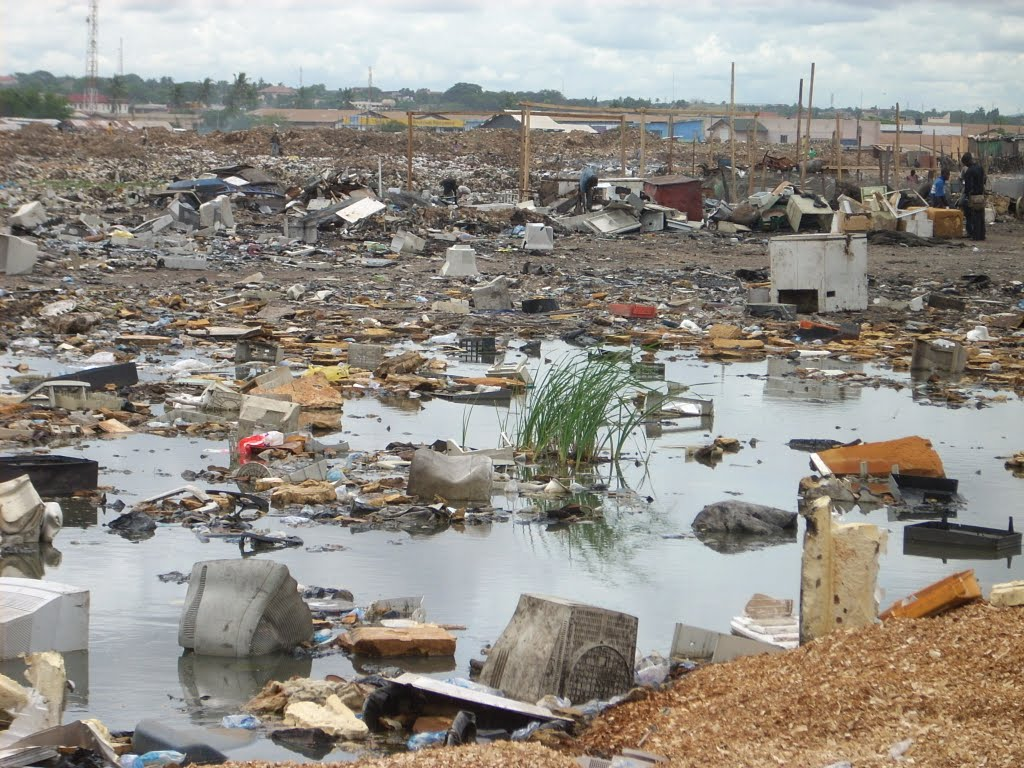
\includegraphics[width=0.5\textwidth]{../inputs/images/ewaste_jack_caravano.jpg}
  \caption{Foto do depósito de lixo eletrônico (\textit{e-waste}) situado no bairro 
           de Agbogbloshie em Acra. Autorizado por Jack Caravanos, 
           Professor da School of Public Health em Hunter College, CUNY
           Nova Iorque, Estado Unidos da América. \label{fig:ewaste}}
\end{figure}

%%%%
\subsection{Nima}

<<<<<<< HEAD
Nima é um dos bairros mais pobres de Acra. É formada de assentamentos não 
planejados, compostos principalmente de migrantes das partes rurais e 
imigrantes de países vizinhos que buscam oportunidades de empregos na capital. 
Com moradias extremamente improvisadas, carece de sistema tratamento de esgoto, 
fornecimento de água potável e eletricidade. 

É conhecida localmente por uma feira de comidas típicas permanentemente 
instalada na região (\textbf{Nima Market}), que é inclusive visitada por turistas.
Com população de origem de diversas partes de Gana, Nima possui 
alta diversidade cultural e religiosa.

O principal meio de transporte dos trabalhadores de Nima para a zona industrial
e de serviços de Acra é feito por vans. 
Muitas vias não são pavimentadas e a intensa movimentação de veículos causa 
levantamento de poeira do solo.

O carvão e a lenha são bastante empregados como fontes de energia para preparação de 
alimentos. A figura \ref{fig:nima} mostra imagens de áreas de cozimento típicas no bairro.

%Nima é um dos bairros mais pobres de Acra e é formada de assentamentos não 
%planejados compostos principalmente de migrantes das partes rurais e 
%imigrantes de países vizinhos que buscam oportunidades de empregos na capital. 
%As moradias são improvisadas e carecem de sistema tratamento de esgoto, 
%fornecimento de água potável e eletricidade. Além disso, muitas vias não são 
%pavimentadas, causando o levantamento de poeira. 

%O meio de transporte dos trabalhadores para realizar o trajeto de suas casas a 
%zona industrial e comercial da cidade é usualmente feito por vans.

%A diversidade de Nima possui alta diversidade
%cultural e religiosa, e é conhecida por uma feira de comidas típicas 
%permanentemente instalada na região, (\textit{The Nima Market}).

%As cozinhas dos moradores de Nima são instalações simples, adaptadas para o uso
%de carvão e lenha como fonte de energia para o cozimento dos alimentos, 
%podendo ser observadas nas imagens da figura \ref{fig:nima}.


\begin{figure}[H]
  \begin{subfigure}[b]{0.5\textwidth}
    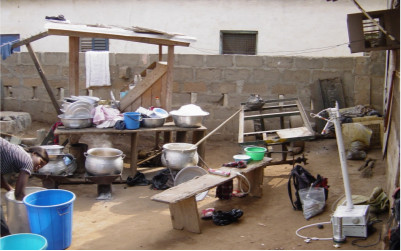
\includegraphics[width=\textwidth]{../inputs/images/zheng/nima1.jpg}
    \caption{}
  \end{subfigure}%
  \begin{subfigure}[b]{0.5\textwidth}
    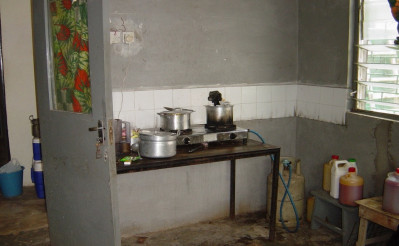
\includegraphics[width=\textwidth]{../inputs/images/zheng/nima2.jpg}
    \caption{}
  \end{subfigure}
  \caption{Fotos de residências de Nima, por Raphael Arku \label{fig:nima}}
\end{figure}
